\documentclass[11pt]{article}
\usepackage[backend=bibtex,style=authoryear,citestyle=authoryear,doi=false,eprint=false]{biblatex}
\usepackage{graphicx, float, hyperref, relsize, multicol, geometry, tikz, caption}
\usepackage[ruled,noline,linesnumbered]{algorithm2e}
\usepackage[utf8]{inputenc}
\usepackage[english]{babel}
\usepackage[T1]{fontenc}
\usetikzlibrary{shapes.geometric, arrows, positioning, fit}
\tikzstyle{process} = [rectangle, minimum width=3cm, minimum height=1cm,text centered, draw=black,text width=4cm, fill=green!30]
\tikzstyle{code} = [rectangle, minimum width=3cm, minimum height=1cm,text centered, draw=black,text width=4cm, fill=green!30]
\tikzstyle{entity} = [rectangle, minimum width=3cm, minimum height=1cm, text centered, draw=black, fill=red!20]
\tikzstyle{arrow} = [thick,->,>=stealth]

 \geometry{
 a4paper,
 total={170mm,257mm},
 left=20mm,
 top=20mm,
 }
\setlength{\columnsep}{1cm}
\graphicspath{ {images/} }
\addbibresource{report.bib}
\title{An interactive tool for designing SKA HI surveys}
\author{Harry Smallbone}

\begin{document}

\maketitle

\section{Introduction}

The Square Kilometre Array (SKA) represents the cutting edge of radio telescope science due to its high sensitivity, low susceptibility to noise effects and large imaging resolution. This will allow HI surveys targeted at much higher redshifts and sensitivity outside of the local universe. An interactive tool that is accessible online is desired to facilitate survey design and to explore the survey parameter space over changing telescopes. The tool has been implemented as a website at \url{http://skaplanner.icrar.org}, and is available publicly. The website is able to display contour and linear plots for: 
\begin{itemize}
\item Redshift
\item Observation time
\item Observation area
\item Physical and Angular Resolution
\item HI column density sensitivity
\item Survey speed
\item RMS noise
\item Predicted number of HI galaxy detections
\end{itemize}
In brief, the website is able to use scaling relations on tables of performance parameters for a number of telescopes to display plots of different survey parameters. 

\section{Background}
HI surveys are a major science goal for the SKA, and there are already preliminary survey designs using predicted performance values \parencite{lister2015}. A major limitation of previous HI surveys such as ALFALFA \parencite{alfalfa} or HIPASS \parencite{hipass2003, hipass2005} has been the low column density of HI gas. HI gas at a density of below $10^{19} cm^{-2}$ is theorised to make up much of the Intergalactic Medium (IGM) and drive galaxy formation \parencite{popping2014}. In order to detect the IGM, telescopes with column density sensitivity on the order of about $ 10^{18} cm^{-2} $ are required, along with enough spatial resolution to resolve structure and kinematics of the HI gas itself.

In order to reach this desired sensitivity, there are a number of parameters which can be tuned depending on the observation volume. An example table of parameters can be seen in Figure \ref{fig:surveytable1}. Specific science goals such as a small observation area of a single galaxy, or an all-sky survey of as many galaxies as possible, have a large impact on how the different parameters should be explored. Often it is necessary to set explicit fixed limits on some parameters and examine how the target parameters such as column density sensitivity change as other parameters vary.
\begin{figure}[H]
    \centering
    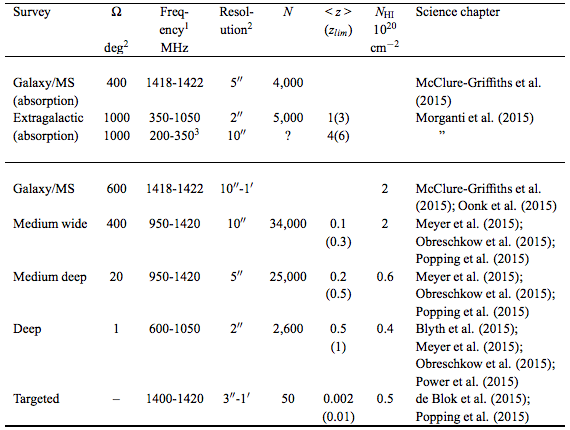
\includegraphics[width=0.75\textwidth]{surveytable1}
    \caption{Sample 1000hr SKA1 H1 surveys \parencite[p. 6]{lister2015}}
    \label{fig:surveytable1}
\end{figure}

An example of this can be seen in Figure \ref{fig:beamss}, a comparison graph of survey speed against beam for different telescopes. These types of comparison graphs are frequently recomputed and changed along with science goals or indeed telescope performance changes as with the SKA rebaselining in 2015. In \textcite{popping2014}, these plots are derived using scaling relations on a MIRIAD simulation of a typical SKA observation day. The MIRIAD simulation has two outputs: a Tsys curve describing atmospheric noise influence at different redshifts of HI, and a table of the effect of synthetic beam size on parameters such as survey speed, noise and HI column density sensitivity.

\begin{figure}[H]
    \centering
    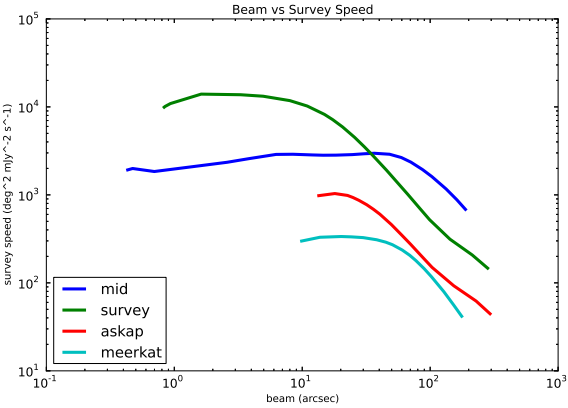
\includegraphics[width=0.75\textwidth]{beamss}
    \caption{Beam against Survey Speed \parencite[p. 6]{popping2014}}
    \label{fig:beamss}
\end{figure}

\section{Software}

\subsection{Tools}

The website has two chief components: a web server and a client which must display plots using scaling relations and equations from \textcite{duffy}.

\subsubsection{Web server}
The web server is written using TurboGears 2 \parencite{turbogears}, a Python program that implements a Model-View-Controller paradigm. The server for the project relies chiefly on scipy \parencite{scipy} to perform integral calculations to predict galaxy detections and solve rotation equations. The server exposes some JSON endpoints to facilitate seamless communication between the client and the server. All telescope performance data is stored on the server.

\subsubsection{Client}
The client is responsible firstly for displaying plots and allowing the user to set various parameters. The client uses Plotly.js \parencite{plotly} and Bootstrap 3 \parencite{bootstrap} respectively for these purposes.

The client also performs the majority of the scaling relations and simple equation solving to avoid placing load on the server for repetitive tasks. These are done inside Web Workers, a newer feature in web browsers that allows asynchronous calculation of large plotting arrays.

\subsubsection{Running the server}
The python requirements to run TurboGears can be set up by executing the \verb|setup.sh| bash script inside the icrar directory. The server can then be run using the \verb|run.sh| file.

\subsection{Algorithms}
As outlined in \textcite{popping2014}, the general approach of the tool is to scale MIRIAD simulation data to obtain values for various parameters and to solve for any missing ones. This is achieved by structuring the program in such a way that four parameters of [NHI, redshift, observation area, observation time and beam resolution] are specified when plotting is required, and the missing parameter can then be solved easily. A full listing of the various cases is available in Algorithms \ref{eqn:scaletables}-\ref{eqn:solverms} (Appendix \ref{sec:algorithms}).

When determining a value for the number of detectable galaxies, the website follows the method outlined in \textcite{duffy}, which uses a HI mass function and simulated galaxy catalogue in order to provide estimates of kinematic profiles and galaxy density needed to arrive at a reasonable detection prediction inside an observation volume. This process is outlined in Algorithm \ref{eqn:solven}. The website makes the following assumptions, mostly in line with the method from \textcite[p. 8]{duffy}.

The diameter of galaxies has been empirically related to HI mass using the relation $$\frac{D_{HI}}{kpc}=\bigg(\frac{M_{HI}}{M_{norm}}\bigg)^\gamma$$ with values $\gamma = 0.55$ and normalisation mass $M_{norm}=10^{6.8}$ \parencite[p. 9]{duffy}.

The inclination of the galaxy to the observer is chosen randomly to match a uniform distribution of $\cos \theta$ \parencite[p. 8]{duffy}.

The velocity width of a galaxy is calculated from the intrinsic line width and $\theta$ value using the relation $$\frac{W_e}{420kms^{-1}}=\bigg(\frac{M_{HI}}{10^{10}}\bigg)^{0.3}$$ where simulating 0.2dex scatter in the relation is shown to be have only an effect of 2\% on the results \parencite[p. 9]{duffy}. This intrinsic line width is converted to a linewidth using angle $\theta$ as chosen earlier and the equation from \textcite{tullyfouque} $$W_e \sin \theta^2 = W_\theta^2 + V_o^2 - 2W_\theta V_o [1-e^{-(\frac{W_\theta}{V_o})^2}] - 2V_o^2e^{-(\frac{W_\theta}{V_o})^2}$$

The chief difference from \textcite{duffy} is the use of a Schechter function \parencite{schechter} from surveys such as \textcite{alfalfa} or \textcite{hipass2003} instead of the simulated galaxy catalogue from that paper. The simulated galaxy catalogue in \textcite{duffy} has a higher resolution in the distribution of $\theta$, the inclination of the galaxy to the observer, due to being able to examine each galaxy individually and a slightly different mass function in low and high mass bins. The website instead uses the number density from the Schechter function to compute a sample of simulated galaxies over many mass bins, which are examined as a group for detection.
\subsection{Program structure}
The website functions primarily as a single page application with limited communication between client and server beyond retrieving MIRIAD simulation data and Schechter integrals. Much of the actual interpolation and solving happens on the client's computer asynchronously. A simple overview flow chart describes this process in Figure \ref{fig:flowchart}.
\begin{figure}[H]
\centering
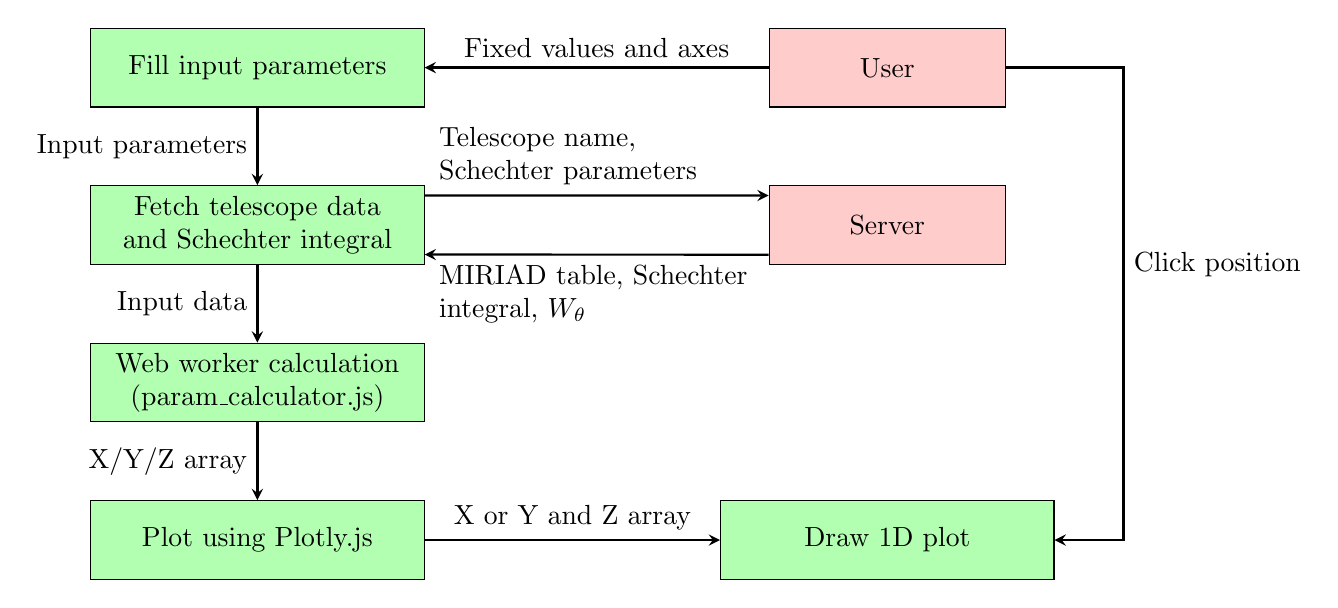
\begin{tikzpicture}[node distance=2cm]
    \node (input) [process] {Fill input parameters};
    \node (fetch) [process, below of=input] {Fetch telescope data and Schechter integral};
    \node (webworker) [process, below of=fetch] {Web worker calculation (param\_calculator.js)};
    \node (plotly) [process, below of=webworker] {Plot using Plotly.js};
    \node (server) [entity, left of=fetch, xshift=10cm] {Server};
    \node (user) [entity, right of=input, xshift=6cm] {User};
    \node (1d) [process, right of=plotly, xshift=6cm] {Draw 1D plot};
    \draw [arrow] (user) -- node[anchor=south] {Fixed values and axes} (input);
    \draw [arrow] (input) -- node[anchor=east] {Input parameters} (fetch);
    \draw [arrow] (fetch.10) -- node[anchor=south, text width=4cm] {Telescope name, Schechter parameters} (server.166);
    \draw [arrow] (server.194) -- node[anchor=north, text width=4cm] {MIRIAD table, Schechter integral, $W_\theta$} (fetch.350);
    \draw [arrow] (fetch) -- node[anchor=east] {Input data} (webworker);
    \draw [arrow] (webworker) -- node[anchor=east] {X/Y/Z array} (plotly);
    \draw [arrow] (plotly) -- node[anchor=south] {X or Y and Z array} (1d);
    \draw [arrow] (user.east) -| (11, 0, 0) node[anchor=west, yshift=-2.5cm] {Click position} |-  (1d.east);
\end{tikzpicture}
\caption{Client program flow chart}
\label{fig:flowchart}
\end{figure}
\begin{figure}[H]
\centering
\resizebox{0.8\textwidth}{!}{%
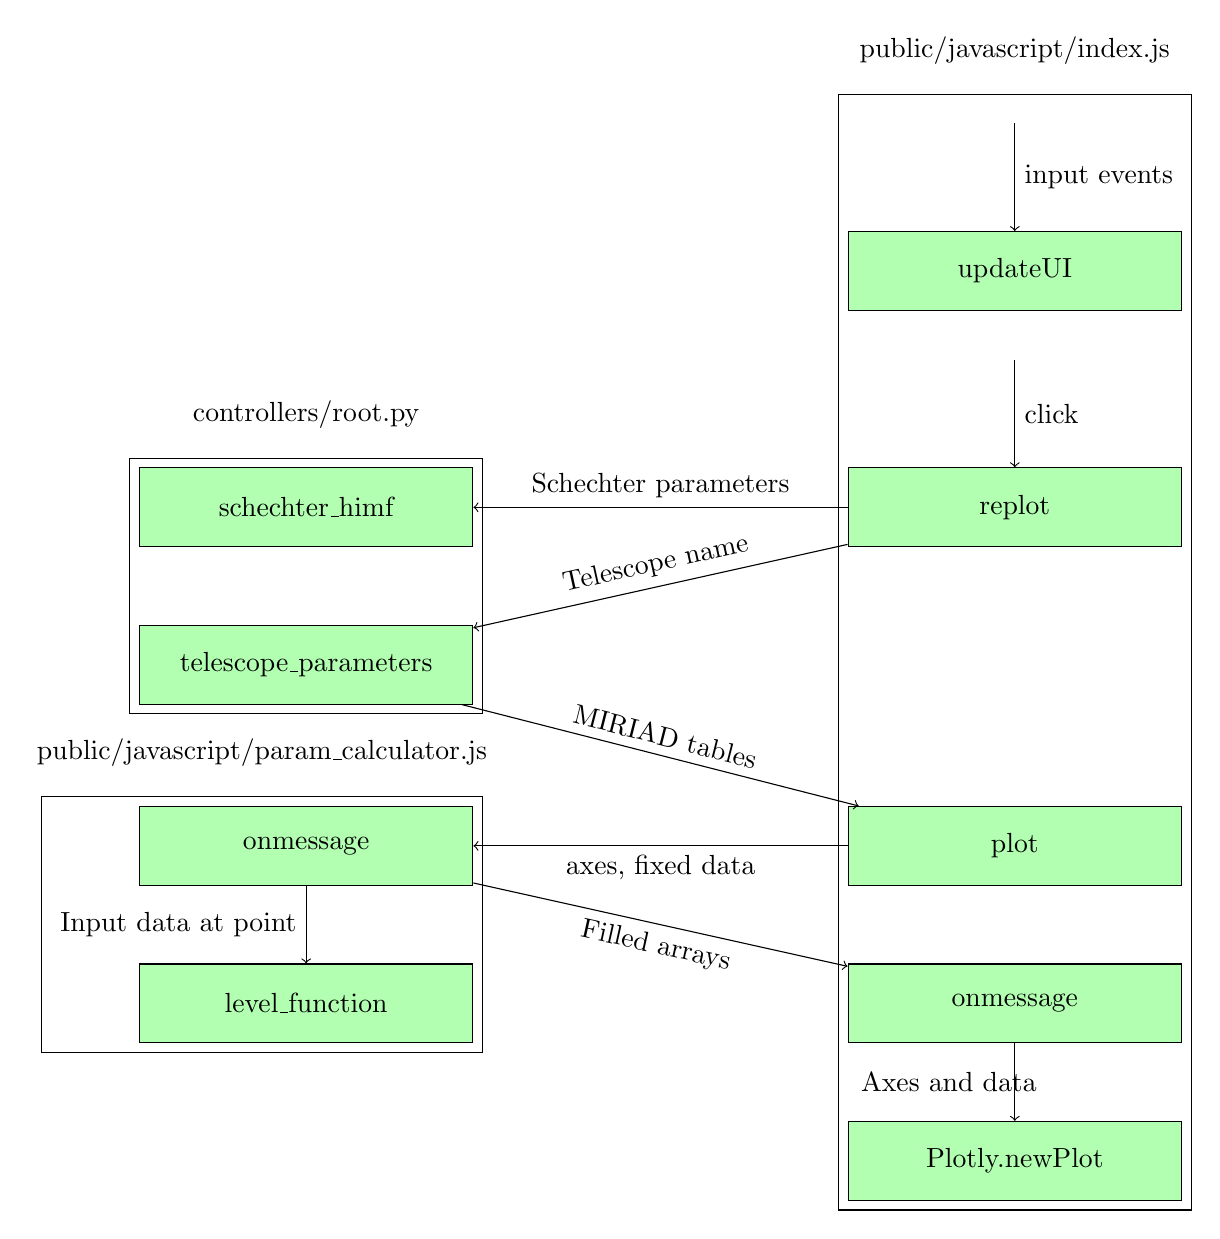
\begin{tikzpicture}[node distance=2cm]
    \node (updateui) [process]{updateUI};
    \node (a1) [draw=none,above of=updateui] {};
    \draw [->] (a1) -- node[auto] {input events} (updateui.north);
    \node(a3) [draw=none,below of=updateui, yshift=1cm] {};
    \node (replot) [code, below of=a3] {replot};
    \draw [->] (a3) -- node[auto]{click} (replot);
    \node (schechter) [code, left of=replot, xshift=-7cm] {schechter\_himf};
    \node (telescope) [code, below of=schechter] {telescope\_parameters};
    \draw [->] (replot) -- node[anchor=south] {Schechter parameters} (schechter);
    \draw [->] (replot) -- node[anchor=south, sloped] {Telescope name} (telescope);
    \node (plot) [code, below of=replot, yshift=-2.3cm] {plot};
    \draw [->] (telescope) -- node[anchor=south,sloped] {MIRIAD tables} (plot);
    \node (wwonmessage) [code, left of=plot, xshift=-7cm] {onmessage};
    \node (levelfunction) [code, below of=wwonmessage] {level\_function};
    \draw [->] (plot) -- node[anchor=north] {axes, fixed data} (wwonmessage);
    \draw [->] (wwonmessage) -- node[anchor=east] (l1) {Input data at point} (levelfunction);
    \node (ionmessage) [code, below of=plot] {onmessage};
    \node (plotly) [code, below of=ionmessage] {Plotly.newPlot};
    \draw [->] (wwonmessage) -- node[anchor=north,sloped] {Filled arrays} (ionmessage);
    \draw [->] (ionmessage) -- node[anchor=east,xshift=0.4cm] {Axes and data} (plotly);
    
    \node[draw=black,fit={(updateui) (a1) (a3) (replot) (plot) (ionmessage) (plotly)},label={[label distance=0.25cm]90:public/javascript/index.js}] {}; 
    \node[draw=black,fit={(schechter) (telescope)},label={[label distance=0.25cm]90:controllers/root.py}] {}; 
    \node[draw=black,fit={(wwonmessage) (l1) (levelfunction)},label={[label distance=0.25cm]90:public/javascript/param\_calculator.js}] {}; 
\end{tikzpicture}
 }%
\caption{Code flow chart}
\label{fig:flowcode}
\end{figure}
\begin{figure}[H]
    \centering
    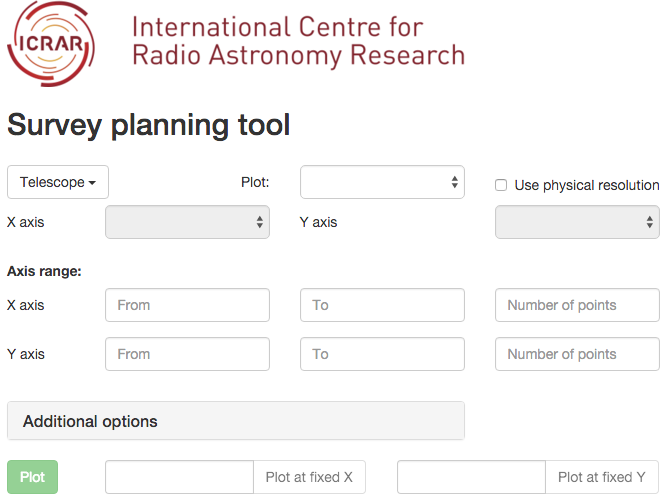
\includegraphics[width=0.75\textwidth]{initialview}
    \caption{Initial view of the index page}
    \label{fig:initialpage}
\end{figure}
The program flow actually starts in the server within TurboGears, where the request is handled inside the root controller under controllers/root.py. This simply renders the HTML template and serves CSS and Javascript files to the client to load the initial webpage. It is important to note that the config/parameters.py file may also be executed to parse the various .telescope files inside the config directory. These .telescope files are described in Appendix \ref{sec:telescopeformat}. The client's web browser produces a page similar to that shown in Figure \ref{fig:initialpage}. At this point Javascript code takes over to wait for changes to the input, inside public/javascript/index.js.

The changes to the interface such as determining which values need to be fixed and input validation are handled by the function \texttt{updateUI}. Once the updateUI function is satisfied that the input is valid, it enables the plot buttons. When these are clicked, the client calls \texttt{replot}, which will fetch the telescope data asynchronously from the server. The server will respond in the methods \verb|schechter_himf| and \verb|telescope_parameters| inside controllers/root.py. Some calculations of Schechter integrals, $\frac{B}{A}$ and $W_e$ are performed inside the \verb|schechter_himf| method to solve equations that are not solvable inside Javascript.

The \texttt{replot} function then creates a Web Worker, which is an asynchronous calculator used to avoid freezing the main webpage while calculations are being performed. The code for the Web Worker begins inside \verb|public/javascript/param_calculator.js|. First, arrays of x, y and z data are created inside the \texttt{onmessage} function. These are spaced on a simple grid given by the user. The arrays are then filled by calling the function \verb|level_function| which solves for the plot parameter. \verb|level_function| performs the majority of the algorithms listed in Appendix \ref{sec:algorithms}. \verb|param_calculator.js| then passes the filled arrays back to \verb|index.js|. 

At this point, the \texttt{plot} function will send the data to Plotly.js, a Javascript plotting library which will actually display the data and handle hover and click events. \texttt{plot} also overrides the default Plotly.js buttons to add a download data button which will download a tab-separated file of the plotting arrays. An overall flow chart of this process is shown in Figure \ref{fig:flowcode}.

\section{Conclusion}
The website is available at \url{http://skaplanner.icrar.org}, and has been deployed using Apache on the ICRAR webservers. The source code for the tool is also available on Github at \url{https://github.com/hsmallbone/ICRAR_Project}.

\appendix
\section{Algorithm listing}
\label{sec:algorithms}
\begin{algorithm}[H]
\DontPrintSemicolon
\KwData{MIRIAD tables, redshift, Tsys table}
\KwResult{Scaled tables at redshift and Tsys}
\Begin{
$conversion\:factor \longleftarrow \sqrt{\frac{1000}{8}}$ \;
\For{$x \in MIRIAD\:table$} {
	$beam[x] \longleftarrow (1 + z) * MIRIAD\:beam[x]$ \;
	$rms[x] \longleftarrow \frac{MIRIAD\:RMS[x]}{conversion\:factor} * Tsys$ \;
	\If{using frequency width} {
		$nhi[x] \longleftarrow \frac{MIRIAD\:NHI[x]}{conversion\:factor} * Tsys * (1 + z)^{1.5}$ \;
	}
	\Else {
		$nhi[x] \longleftarrow \frac{MIRIAD\:NHI[x]}{conversion\:factor} * Tsys * (1 + z)^{2}$ \;
	}
	$ss[x] \longleftarrow \frac{MIRIAD\:SS[x]}{conversion\:factor} * Tsys^2 * (1 + z)^2$ \;
}
\caption{Scale MIRIAD tables\label{eqn:scaletables}}
}
\end{algorithm}
\begin{algorithm}[H]
\DontPrintSemicolon
\KwData{Synthetic beam size, tables from Algorithm \ref{eqn:scaletables}, frequency width and observation time}
\KwResult{NHI column density sensitivity}
\Begin{
$\log_{10} beamsize \longleftarrow \log_{10} synthetic\:beamsize$\;
$NHI (1000hr, 50kHz) \longleftarrow lerp(\log_{10} beam[], \log_{10} NHI[])$\;
$NHI (1000hr) \longleftarrow \log_{10}\sqrt{\frac{frequency\:width}{50kHz}} + NHI (1000hr, 50kHz)$\;
$NHI \longleftarrow NHI (1000hr) - \frac{\log_{10}(observation\:time\:(single\:pointing) / 1000)}{2}$\;
\caption{Solve NHI\label{eqn:solvenhi}}
}
\end{algorithm}
\begin{algorithm}[H]
\DontPrintSemicolon
\KwData{Redshift, dish size, observation area, tables from Algorithm \ref{eqn:scaletables}}
\KwResult{Observation time}
\Begin{
$\Theta_p \longleftarrow 1.22 * (1 + z) * \frac{\frac{c * 1000}{HI_{freq}}}{dishsize} * \frac{180}{\pi}$ \;
$\Omega_b \longleftarrow 0.5665 * \Theta_p^2$ \;
$n_{pointings} \longleftarrow \frac{area}{\Omega_b}$ \;
$\log_{10}beam \longleftarrow \log_{10} synthetic\:beamsize$ \;
$NHI (1000hr, 50kHz) \longleftarrow lerp(\log_{10} beam[], \log_{10} NHI[])$\;
$NHI (1000hr) \longleftarrow \log_{10}\sqrt{\frac{frequency\:width}{50kHz}} + NHI (1000hr, 50kHz)$\;
$time_{single\:pointing} \longleftarrow 1000 * 10^{2 * (NHI(1000hr) - NHI (desired))}$ \;
$time_{total} \longleftarrow time_{single\:pointing} * n_{pointings}$ \;
\caption{Solve observation time\label{eqn:solvetime}}
}
\end{algorithm}
\begin{algorithm}[h!]
\DontPrintSemicolon
\KwData{Frequency width, observation time (single pointing), tables from Algorithm \ref{eqn:scaletables}}
\KwResult{Beam resolution}
\Begin{
$NHI (1000hr) \longleftarrow 0.5 * \log_{10} \frac{observation\:time}{1000} + NHI (desired)$ \;
$NHI (1000hr, 50kHz) \longleftarrow NHI (1000hr) - \log_{10} \sqrt{\frac{frequency\:width}{50kHz}}$ \;
$\log_{10} synthetic\:beamsize \longleftarrow lerp(NHI (1000hr, 50kHz), \log_{10} NHI, \log_{10} beamsize) $ \;
$resolution \longleftarrow 10^{\log_{10} synthetic\:beamsize}$ \;
\caption{Solve beam resolution\label{eqn:solvebeam}}
}
\end{algorithm}
\begin{algorithm}[h!]
\DontPrintSemicolon
\KwData{Tables from Algorithm \ref{eqn:scaletables}, desired NHI sensitivity}
\KwResult{Maximum resolvable redshift}
\Begin{
\For{$z \leftarrow 0$ \KwTo $20$} {
	Scale MIRIAD tables to redshift $z$ \;
	$NHI (1000hr) \longleftarrow 0.5 * \log_{10} \frac{observation\:time}{1000} + NHI (desired)$ \;
	$NHI (1000hr, 50kHz) \longleftarrow NHI (1000hr) - \log_{10} \sqrt{\frac{frequency\:width}{50kHz}}$ \;
	$Resolvable \:NHI (1000hr, 50kHz) \longleftarrow lerp(\log_{10} synthetic\:beamsize, \log_{10} beamsize, \log_{10} NHI) $ \;
	\If {$NHI (1000hr, 50kHz) > Resolvable\:NHI (1000hr, 50kHz)$} {
		$max(z) \longleftarrow z$ \;
	} \Else {
		break \;
	}
}
\caption{Solve maximum resolvable redshift\label{eqn:solveredshift}}
}
\end{algorithm}
\begin{algorithm}[h!]
\DontPrintSemicolon
\KwData{Tables from Algorithm \ref{eqn:scaletables}, synthetic beam size, frequency width}
\KwResult{Survey speed}
\Begin{
$SS (1000hr, 50kHz) \longleftarrow lerp(log_{10} synthetic\:beamsize, log_{10} beamsize[], SS[])$ \;
$SS \longleftarrow SS (1000hr, 50kHz) * \sqrt{\frac{50kHz}{frequency\:width}}$ \;
\caption{Solve survey speed\label{eqn:solvess}}
}
\end{algorithm}
\begin{algorithm}[h!]
\DontPrintSemicolon
\KwData{Tables from Algorithm \ref{eqn:scaletables}, synthetic beamsize, frequency width, observation time}
\KwResult{Observation time}
\Begin{
$RMS (1000hr, 50kHz) \longleftarrow lerp(log_{10} synthetic\:beamsize, log_{10} beamsize[], RMS[])$ \;
$RMS (1000hr) \longleftarrow RMS (1000hr, 50kHz) * \sqrt{\frac{50kHz}{frequency\:width}}$ \;
$RMS \longleftarrow RMS (1000hr) * \sqrt{\frac{1000}{observation\:time_{single\:pointing}}}$ \;
\caption{Solve RMS\label{eqn:solverms}}
}
\end{algorithm}
\begin{algorithm}[H]
\DontPrintSemicolon
\KwData{Tables from Algorithm \ref{eqn:scaletables}, synthetic beamsize, redshift range, Schechter mass function parameters}
\KwResult{Estimated number of HI galaxy detections}
\Begin{
luminosity distance $\longleftarrow (1 + z) * comoving\_distance(z_1)$ \;
angular diameter distance $\longleftarrow \frac{comoving\_distance(z_1)}{1+z}$ \;
$RMS (1000hr, 50kHz) \longleftarrow lerp(log_{10} synthetic\:beamsize, log_{10} beamsize[], RMS[])$ \;
$RMS (1000hr) \longleftarrow RMS (1000hr, 50kHz) * \sqrt{\frac{50kHz}{frequency\:width}}$ \;
$RMS \longleftarrow RMS (1000hr) * \sqrt{\frac{1000}{observation\:time_{single\:pointing}}}$ \;
$\sigma_v \longleftarrow$ frequency width $(kms^{-1})$ \;
Observation volume (MPC) $\longleftarrow comoving\_volume(z_0, z_1)$ \;
\For {$M_{HI0}, M_{HI1} \in$ Schechter table} {
	$M_{HI} \longleftarrow 10^{midpoint(M_{HI0}, M_{HI1})}$ \;
	$integral \longleftarrow \mathlarger{\int_{log_{10} M_{HI0}}^{log_{10} M_{HI1}} \ln 10 * \phi_* (\frac{M_{HI}}{M_*})^{\alpha + 1} e^{-\frac{M_{HI}}{M_*}}}$ \;
	$\theta_{inclination} \longleftarrow acos($random cos from 0.12-0.88 $)$ \;
	$\frac{B}{A} \longleftarrow \sqrt{\cos \theta_{inclination}^2 * (1 - 0.12) + 0.12} $ \;
	$\omega_e \longleftarrow 420 * (\frac{M_{HI}}{10^{10}})^{0.3}$ \;
	$V_o \longleftarrow 20 kms^{-1}$ \;
	$V_c \longleftarrow 120 kms^{-1}$ \;
	$W_\theta \longleftarrow solve\:(W_e \sin \theta^2 = W_\theta^2 + V_o^2 - 2W_\theta V_o [1-e^{-(\frac{W_\theta}{V_o})^2}] - 2V_o^2e^{-(\frac{W_\theta}{V_o})^2})$ \;
	$N_{chans} \longleftarrow \frac{W_\theta}{\sigma_v}$ \;
	$D_{HI} (kpc) \longleftarrow \mathlarger{\bigg(\frac{M_{HI}}{10^{6.8}}\bigg)^{0.55}}$ \;
	Angular size $(arcsec^2) \longleftarrow \frac{D_{HI}}{angular\:diameter\:distance} * \frac{180}{\pi} * 60^2$ \;
	$A_{gal} \longleftarrow \pi * (\frac{Angular\:size}{2})^2 * \frac{B}{A}$ \;
	$A_{beam} \longleftarrow \frac{\pi * synthetic\:beamsize^2}{4 \ln 2}$ \;
	$S_{tot} \longleftarrow \frac{M_{HI}}{49.8} * luminosity\:distance^{-2}$ \;
	$\frac{S}{N} \longleftarrow \mathlarger{\frac{S_{tot}}{\sigma_{chan} * \sigma_v * \sqrt{N_{chans}} * \sqrt{1 + \frac{A_{gal}}{A_{beam}}}}}$ \;
	\If{$\frac{S}{N} > \frac{S}{N}\:limit$} {
		$n \longleftarrow n + integral * observation\:volume$ \;
	}
}
\caption{Predict number of detectable HI galaxies\label{eqn:solven}}
}
\end{algorithm}
\section{.telescope file format}
\label{sec:telescopeformat}
All .telescope files inside the config/ directory are loaded to produce a set of available telescope performance parameters for the user. The format is relatively simple:

\begin{verbatim}
Telescope name
Dish size
List of: Beam size (arcsec), RMS noise (mJy), 
NHI column density sensitivity (cm^-2), survey speed
tsys
Tab separated list of: HI frequency, Ae/Tsys
\end{verbatim}
where the Tsys curve is optional and will default to the curve specified in config/tsys.cfg if not given. \subsection{Example for SKA1-MID}
\begin{verbatim}
SKAMID
15 
0.432330275229 0.104589473684 6.48242235182e+21 1371.8502756
0.472468487395 0.102718421053 5.33605158544e+21 1422.28293738
0.698041399001 0.106839473684 2.55266547487e+21 1314.67737836
1.3309838891 0.100693421053 6.62309834748e+20 1480.06393926
tsys
0.363	2.386
0.369	2.47025
0.376	2.564
0.384	2.65575
0.392	2.7595
\end{verbatim}
\subsection{Adding a new telescope}
A new telescope file can be added at any time by putting a new .telescope file inside the config/ directory. Python will automatically load it and send it to the client.
\section{Adding a new plot parameter}
\begin{enumerate}
\item Add a new short name to the \verb|possible_plot_parameters| array in \verb|index.js|.
\item Add a new entry inside the \verb|param_info| dictionary to describe the units and name of the new parameter.
\item Implement a new else if case inside \verb|param_calculator.js| for the new short parameter name.
\end{enumerate}

\section{Bibliography}
\printbibliography
\end{document}
